\documentclass{article}

%========================================================================================
% PREAMBLE
% This section defines the document's overall style and includes necessary packages.
%========================================================================================
\usepackage[letterpaper, margin=1in, textwidth=6.5in]{geometry}
\usepackage{graphicx}
\usepackage{amsmath}
\usepackage{amssymb}
\usepackage{amsfonts}
\usepackage{enumitem}
\usepackage{pdfpages}
\usepackage{chemformula}    % For chemical formulas like \ch{H2O}
\usepackage{siunitx}        % For units like \SI{8.82e-4}{M}
\usepackage{hyperref}       % For clickable links (optional)
\hypersetup{colorlinks=true, linkcolor=blue, urlcolor=cyan}

%========================================================================================
% DOCUMENT METADATA
%========================================================================================
\title{Comprehensive Study Guide for Chapter 9 Quiz}
\author{}
\date{}

\begin{document}

\maketitle % This generates the title.
\pagenumbering{gobble} % Removes page numbering for a clean look.

% ---------------------------------------------------------------------------------------------------
% SECTION 1: QUIZ DETAILS AND TOPICS
% ---------------------------------------------------------------------------------------------------
\hrulefill
\subsection*{Quiz Details}
\begin{itemize}[itemsep=5pt] % 'itemsep=5pt' adds vertical space between list items.
    \item \textbf{Date and Time:} Tuesday, October 21st, between 7:00 AM and 7:30 AM.
    \item \textbf{Format:} Closed notes.
    \item \textbf{Allowed Materials:} A scientific calculator.
\end{itemize}

\hrulefill
\subsection*{Key Topics on the Quiz}
\begin{enumerate}[itemsep=5pt]
    \item Using the provided solubility rules to determine if an ionic compound is soluble or insoluble.
    \item Calculating the pH given [\ch{H3O+}] concentration, applying significant figure rules, and classifying the solution as acidic, basic, or neutral.
    \item Stating the oxidation number of an atom in a compound or element (must know the 7 rules by heart).
    \item Balancing a redox reaction using either the half-reaction method or the visual method.
\end{enumerate}
\hrulefill
\bigskip % Adds a larger vertical space.

% ---------------------------------------------------------------------------------------------------
% SECTION 2: PHASED STUDY PLAN
% ---------------------------------------------------------------------------------------------------
\section*{Phased Study Plan}

\subsection*{Phase 1: Foundation \& Memorization (Friday - Saturday)}
\begin{itemize}[itemsep=5pt]
    \item \textbf{Memorize Oxidation Rules:} Your first priority is to memorize the seven rules for assigning oxidation numbers. This is a non-negotiable requirement for the quiz.
    \begin{itemize}
        \item \textbf{Source:} \texttt{Chapter 9 Chemical reactions in aqueous solutions.pdf}, \textbf{Slides 48 \& 49}. Create flashcards or use mnemonic devices.
    \end{itemize}
    \item \textbf{Understand Core Concepts:} Review the PowerPoint slides to build a strong foundation for each topic.
    \begin{itemize}
        \item \textbf{Solubility:} Understand the terms soluble and insoluble. Review the table on \textbf{Slide 34}.
        \item \textbf{pH Concept:} Understand the logarithmic relationship between pH and [\ch{H3O+}]. Review \textbf{Slides 16-19}. Pay special attention to the significant figure rule on Slide 17.
        \item \textbf{Redox Reactions:} Learn the definitions of oxidation and reduction. Review the half-reaction method on \textbf{Slides 58-59}.
    \end{itemize}
\end{itemize}

\subsection*{Phase 2: Practice \& Application (Saturday - Sunday)}
\begin{itemize}[itemsep=5pt]
    \item \textbf{Solubility Practice:}
    \begin{itemize}
        \item Work through problems \textbf{9.22} and \textbf{9.23} on page 404 of the \texttt{Questions and Problems} PDF. Use the table on Slide 34 to determine your answers.
    \end{itemize}
    \item \textbf{pH Calculation Drills:}
    \begin{itemize}
        \item Complete problems \textbf{9.80} and \textbf{9.81} on page 407 of the \texttt{Questions and Problems} PDF. Write down the pH, your reasoning for the number of decimal places, and whether it's acidic or basic.
    \end{itemize}
    \item \textbf{Oxidation Number Drills:}
    \begin{itemize}
        \item Complete the entire \texttt{Oxidation states and redox reactions.pdf} worksheet (Part 1). This is the best way to master the 7 rules.
        \item For more practice, solve problems \textbf{9.49}, \textbf{9.50}, and \textbf{9.51} on page 405 of the \texttt{Questions and Problems} PDF.
    \end{itemize}
\end{itemize}

\subsection*{Phase 3: Final Mastery (Monday)}
\begin{itemize}[itemsep=5pt]
    \item \textbf{Balance Redox Reactions:}
    \begin{itemize}
        \item Work through all problems in \textbf{Part 3} of the \texttt{Oxidation states and redox reactions.pdf} worksheet. This gives you direct practice with the half-reaction method.
    \end{itemize}
    \item \textbf{Review Explanations:} Carefully read the detailed walkthroughs in the next section of this guide. Compare your work to the correct methods.
    \item \textbf{Self-Correction:} Redo any problems you got wrong in Phase 2 without looking at the answers. The goal is to be able to solve them correctly and confidently on your own.
    \item \textbf{Final Check:} Get a good night's sleep. Make sure your calculator is ready.
\end{itemize}
\newpage

% ---------------------------------------------------------------------------------------------------
% SECTION 3: EXPLANATIONS OF KEY TOPICS
% ---------------------------------------------------------------------------------------------------
\section*{Explanations of Key Topics and Practice Problems}

\subsection*{Topic 1: Using Solubility Rules}
\textbf{Goal:} To classify an ionic compound as soluble or insoluble based on the provided rules.
\begin{itemize}[itemsep=5pt]
    \item \textbf{Reference:} \texttt{Chapter 9...pdf}, Slide 34, TABLE 4.1
\end{itemize}
\subsubsection*{Example: Classify \ch{AgCl} and \ch{Na3PO4}.}
\begin{enumerate}[label=\textbf{Step \arabic*:}, itemsep=5pt]
    \item \textbf{Classify \ch{AgCl}:}
    \begin{itemize}
        \item \textbf{Identify Ions:} Ag$^{+}$ and Cl$^{-}$.
        \item \textbf{Apply Rule:} Find the Cl$^{-}$ ion in the "Generally Soluble" section. Check its exceptions. The exceptions state that when Cl$^{-}$ pairs with Ag$^{+}$, the compound is insoluble.
        \item \textbf{Conclusion:} \ch{AgCl} is \textbf{insoluble}.
    \end{itemize}
    \item \textbf{Classify \ch{Na3PO4}:}
    \begin{itemize}
        \item \textbf{Identify Ions:} Na$^{+}$ and PO$_4^{3-}$.
        \item \textbf{Apply Rule:} Find the PO$_4^{3-}$ ion in the "Generally Insoluble" section. Check its exceptions. The exceptions state that when PO$_4^{3-}$ pairs with Na$^{+}$ (an alkali metal ion), the compound is soluble.
        \item \textbf{Conclusion:} \ch{Na3PO4} is \textbf{soluble}.
    \end{itemize}
\end{enumerate}

\subsection*{Topic 2: Calculating pH}
\textbf{Goal:} To calculate pH from [\ch{H3O+}] with correct significant figures and classify the solution.
\begin{itemize}[itemsep=5pt]
    \item \textbf{Reference:} \texttt{Chapter 9...pdf}, Slides 17-19
\end{itemize}
\subsubsection*{Key Formula and Rule:}
\[ \text{pH} = -\log[\ch{H3O+}] \]
\textbf{Sig Fig Rule:} The number of \textbf{decimal places} in the pH must equal the number of \textbf{significant figures} in the [\ch{H3O+}] concentration.

\subsubsection*{Example Problem (from Slide 19): Calculate the pH for [\ch{H3O+}] = \SI{8.82e-4}{M}.}
\begin{enumerate}[label=\textbf{Step \arabic*:}, itemsep=5pt]
    \item \textbf{Identify Significant Figures:} The concentration, \num{8.82e-4}, has \textbf{three} significant figures (8, 8, 2).
    \item \textbf{Apply the Rule:} The final pH value must be reported to \textbf{three} decimal places.
    \item \textbf{Calculate the pH:}
    \[ \text{pH} = -\log(8.82 \times 10^{-4}) = 3.0544... \]
    \item \textbf{Round to Correct Decimal Places:} Rounding to three decimal places gives \textbf{3.054}.
    \item \textbf{Classify:} Since 3.054 is less than 7, the solution is \textbf{acidic}.
\end{enumerate}

\subsection*{Topic 3: Stating Oxidation Numbers}
\textbf{Goal:} To determine the oxidation number of a specific atom in a compound or ion using the 7 rules.
\begin{itemize}[itemsep=5pt]
    \item \textbf{Reference:} \texttt{Chapter 9...pdf}, Slides 48-49 (Rules), 52-54 (Examples)
\end{itemize}
\subsubsection*{Example Problem (from Slide 53): Determine the oxidation number of Cr in \ch{Na2Cr2O7}.}
\begin{enumerate}[label=\textbf{Step \arabic*:}, itemsep=5pt]
    \item \textbf{Assign Known Oxidation Numbers:}
    \begin{itemize}
        \item Na is a Group 1 metal, so its oxidation number is \textbf{+1} (Rule 2 for ions in compounds).
        \item O has an oxidation number of \textbf{-2} (Rule 3).
    \end{itemize}
    \item \textbf{Set Up an Algebraic Equation:} The compound is neutral, so the sum of all oxidation numbers must be zero (Rule 6). Let the oxidation number of Cr be `x`. Since there are two Cr atoms, we use `2x`.
    \[ \underbrace{2(\text{Na})}_{\text{charge from Na}} + \underbrace{2(\text{Cr})}_{\text{charge from Cr}} + \underbrace{7(\text{O})}_{\text{charge from O}} = 0 \]
    \[ 2(+1) + 2(x) + 7(-2) = 0 \]
    \item \textbf{Solve for x:}
    \begin{align*}
        2 + 2x - 14 &= 0 \\
        2x - 12 &= 0 \\
        2x &= +12 \\
        x &= +6
    \end{align*}
\end{enumerate}
\textbf{Answer:} The oxidation number of each chromium (Cr) atom is \textbf{+6}.

\subsection*{Topic 4: Balancing Redox Reactions}
\textbf{Goal:} To balance a redox equation, ensuring that both atoms and charge are conserved.
\begin{itemize}[itemsep=5pt]
    \item \textbf{Reference:} \texttt{Chapter 9...pdf}, Slides 58-61
\end{itemize}
\subsubsection*{Example Problem (from Slide 59): Balance \ch{Cr(s) + Ni^2+(aq) -> Cr^3+(aq) + Ni(s)}}
\begin{enumerate}[label=\textbf{Step \arabic*:}, itemsep=5pt]
    \item \textbf{Split into Half-Reactions:} Identify what is being oxidized (oxidation number increases) and what is being reduced (oxidation number decreases).
    \begin{itemize}
        \item Cr goes from 0 to +3 (loss of e$^{-}$), so it is \textbf{oxidation}.
        \item Ni goes from +2 to 0 (gain of e$^{-}$), so it is \textbf{reduction}.
    \end{itemize}
    \begin{align*}
        \text{Oxidation:} & \quad \ch{Cr(s) -> Cr^3+(aq)} \\
        \text{Reduction:} & \quad \ch{Ni^2+(aq) -> Ni(s)}
    \end{align*}
    \item \textbf{Balance Charge with Electrons:} Add electrons to the more positive side of each equation.
    \begin{align*}
        \text{Oxidation:} & \quad \ch{Cr(s) -> Cr^3+(aq) + 3e-} \\
        \text{Reduction:} & \quad \ch{Ni^2+(aq) + 2e- -> Ni(s)}
    \end{align*}
    \item \textbf{Equalize Electrons:} The least common multiple of 3 electrons (lost) and 2 electrons (gained) is 6.
    \begin{itemize}
        \item Multiply the oxidation half-reaction by \textbf{2}.
        \item Multiply the reduction half-reaction by \textbf{3}.
    \end{itemize}
    \begin{align*}
        \text{Oxidation } (\times 2): & \quad \ch{2Cr(s) -> 2Cr^3+(aq) + 6e-} \\
        \text{Reduction } (\times 3): & \quad \ch{3Ni^2+(aq) + 6e- -> 3Ni(s)}
    \end{align*}
    \item \textbf{Combine and Cancel:} Add the two new half-reactions together and cancel the species that appear on both sides (the electrons).
    \[ \ch{2Cr(s) + 3Ni^2+(aq) + 6e- -> 2Cr^3+(aq) + 3Ni(s) + 6e-} \]
\end{enumerate}
\textbf{Final Balanced Equation:} \[\ch{2Cr(s) + 3Ni^2+(aq) -> 2Cr^3+(aq) + 3Ni(s)}\]

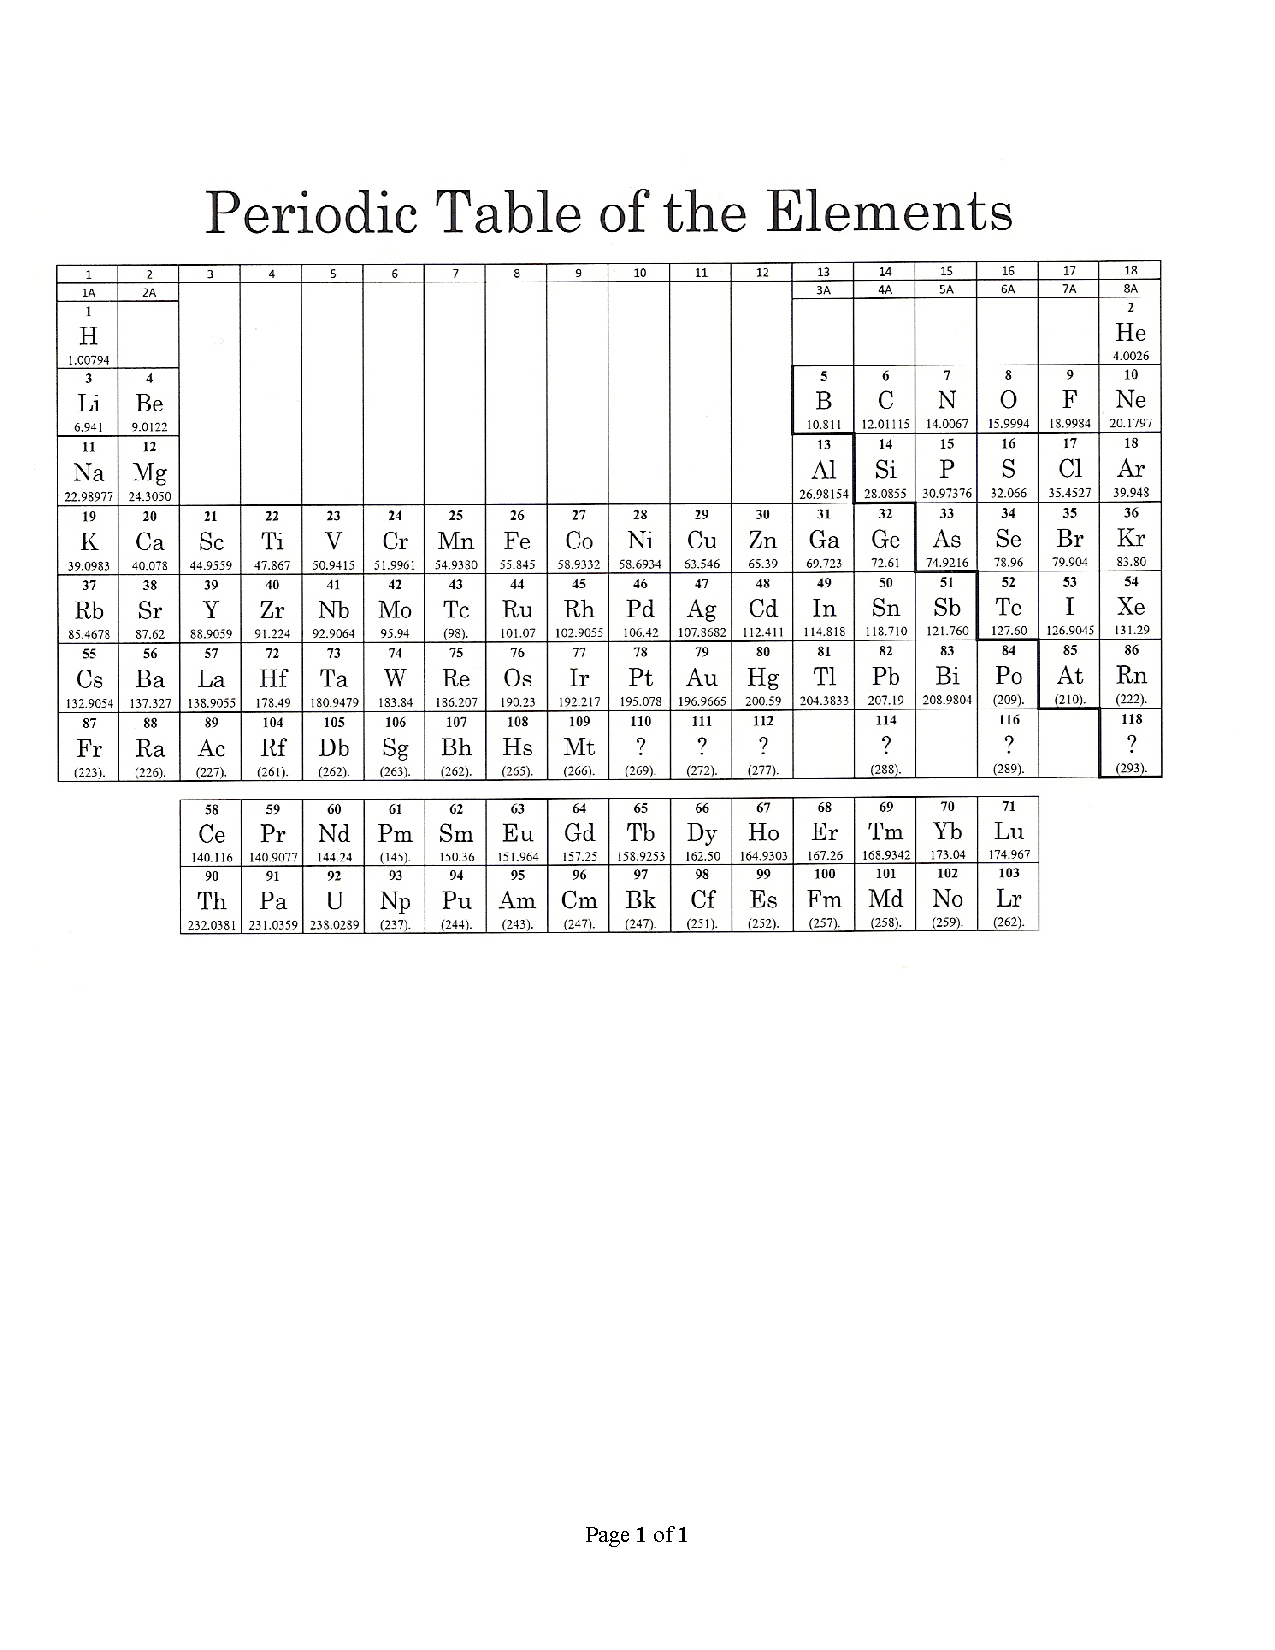
\includepdf[pages={-}]{Periodic Table for testing.pdf}

\end{document}